\chapter{Interfejs użytkownika} 

Ten rozdział zawiera schemat interfejsu użytkownika.

\section{Menu główne}

Na rysunku 7.1 przedstawiony został schematyczny widok menu głównego. 
Z tego menu będzie można wybrać podmenu zapisanych rozgrywek za pomocą przycisku \textit{Kontynuuj rozgrywkę}, rozpocząć nową rozgrywkę za pomocą przycisku \textit{Nowa gra}, przejść do menu ustawień oraz wyjść z gry.

\begin{figure}[H]
    \centering
        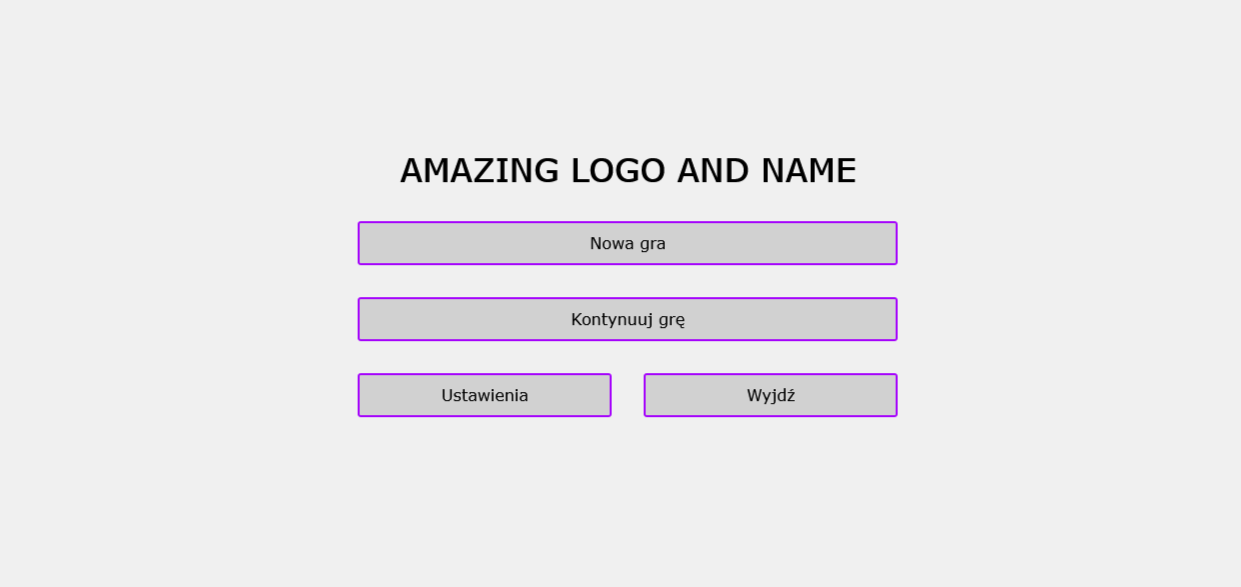
\includegraphics[width=0.9\textwidth]{Graphics/interface/main_menu.png}
        \index{Schemat menu głównego}
        \caption{Schemat menu głównego}
\end{figure}

\section{Interfejs HUD}

Na rysunku 7.2 przedstawiony został schematyczny widok HUD.
HUD będzie wyświetlał obecny poziom zdrowia, temperatury oraz głodu gracza.

\begin{figure}[H]
    \centering
        
\includegraphics[width=0.9\textwidth]{Graphics/interface/HUD.png}
        \index{Schemat HUD}
        \caption{Schemat HUD}
\end{figure}

\section{Menu budowania}

Na rysunku 7.3 przedstawiony został schematyczny widok menu budowania.
W menu budowania będzie można wybrać strukturę do budowy. Przy strukturze będą wyświetlone materiały niezbędne do budowy. To menu będzie umożliwiało wybranie struktury, którą gracz chce zbudować.

\begin{figure}[H]
    \centering
        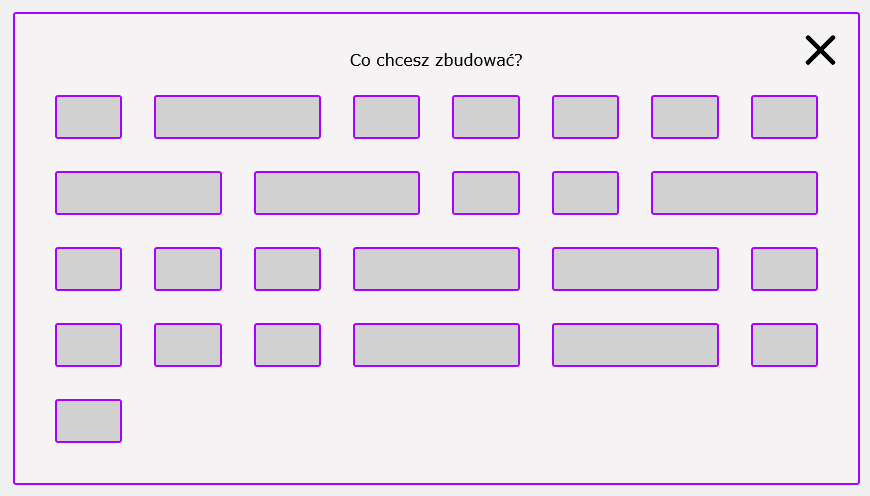
\includegraphics[width=0.9\textwidth]{Graphics/interface/building_menu.png}
        \index{Schemat menu budowania}
        \caption{Schemat menu budowania}
\end{figure}